\subsection{Sandbox}
The application also includes a sandbox page, where students can practice the different question types. The content of the Sandbox component changes depending on the selected question type. The question type select element is mounted to the data property \code{questionType}. Depending on the value given to the \code{questionType} data property, the component content changes in order to accommodate the selected question type. This is done by using \code{v-if}. Question type Text is the default value for the select element. The only component used in the Sandbox view is the GraphDrawer.
\\[11pt]
The elements that are needed for a question type are always displayed in the middle of the page in its own container. The \code{getShowSettings} function is responsible for revealing the settings section when it is required; otherwise, the function is responsible for removing the section altogether.  The content in settings is determined by the question type and uses the same v-if system as the earlier segments. The guide and settings sections are also mounted to their own property called \code{showGuide} and \code{showSettings}. These properties determine whether the content in these sections are displayed or hidden to the user.

\begin{figure}[H]
	\centering	
	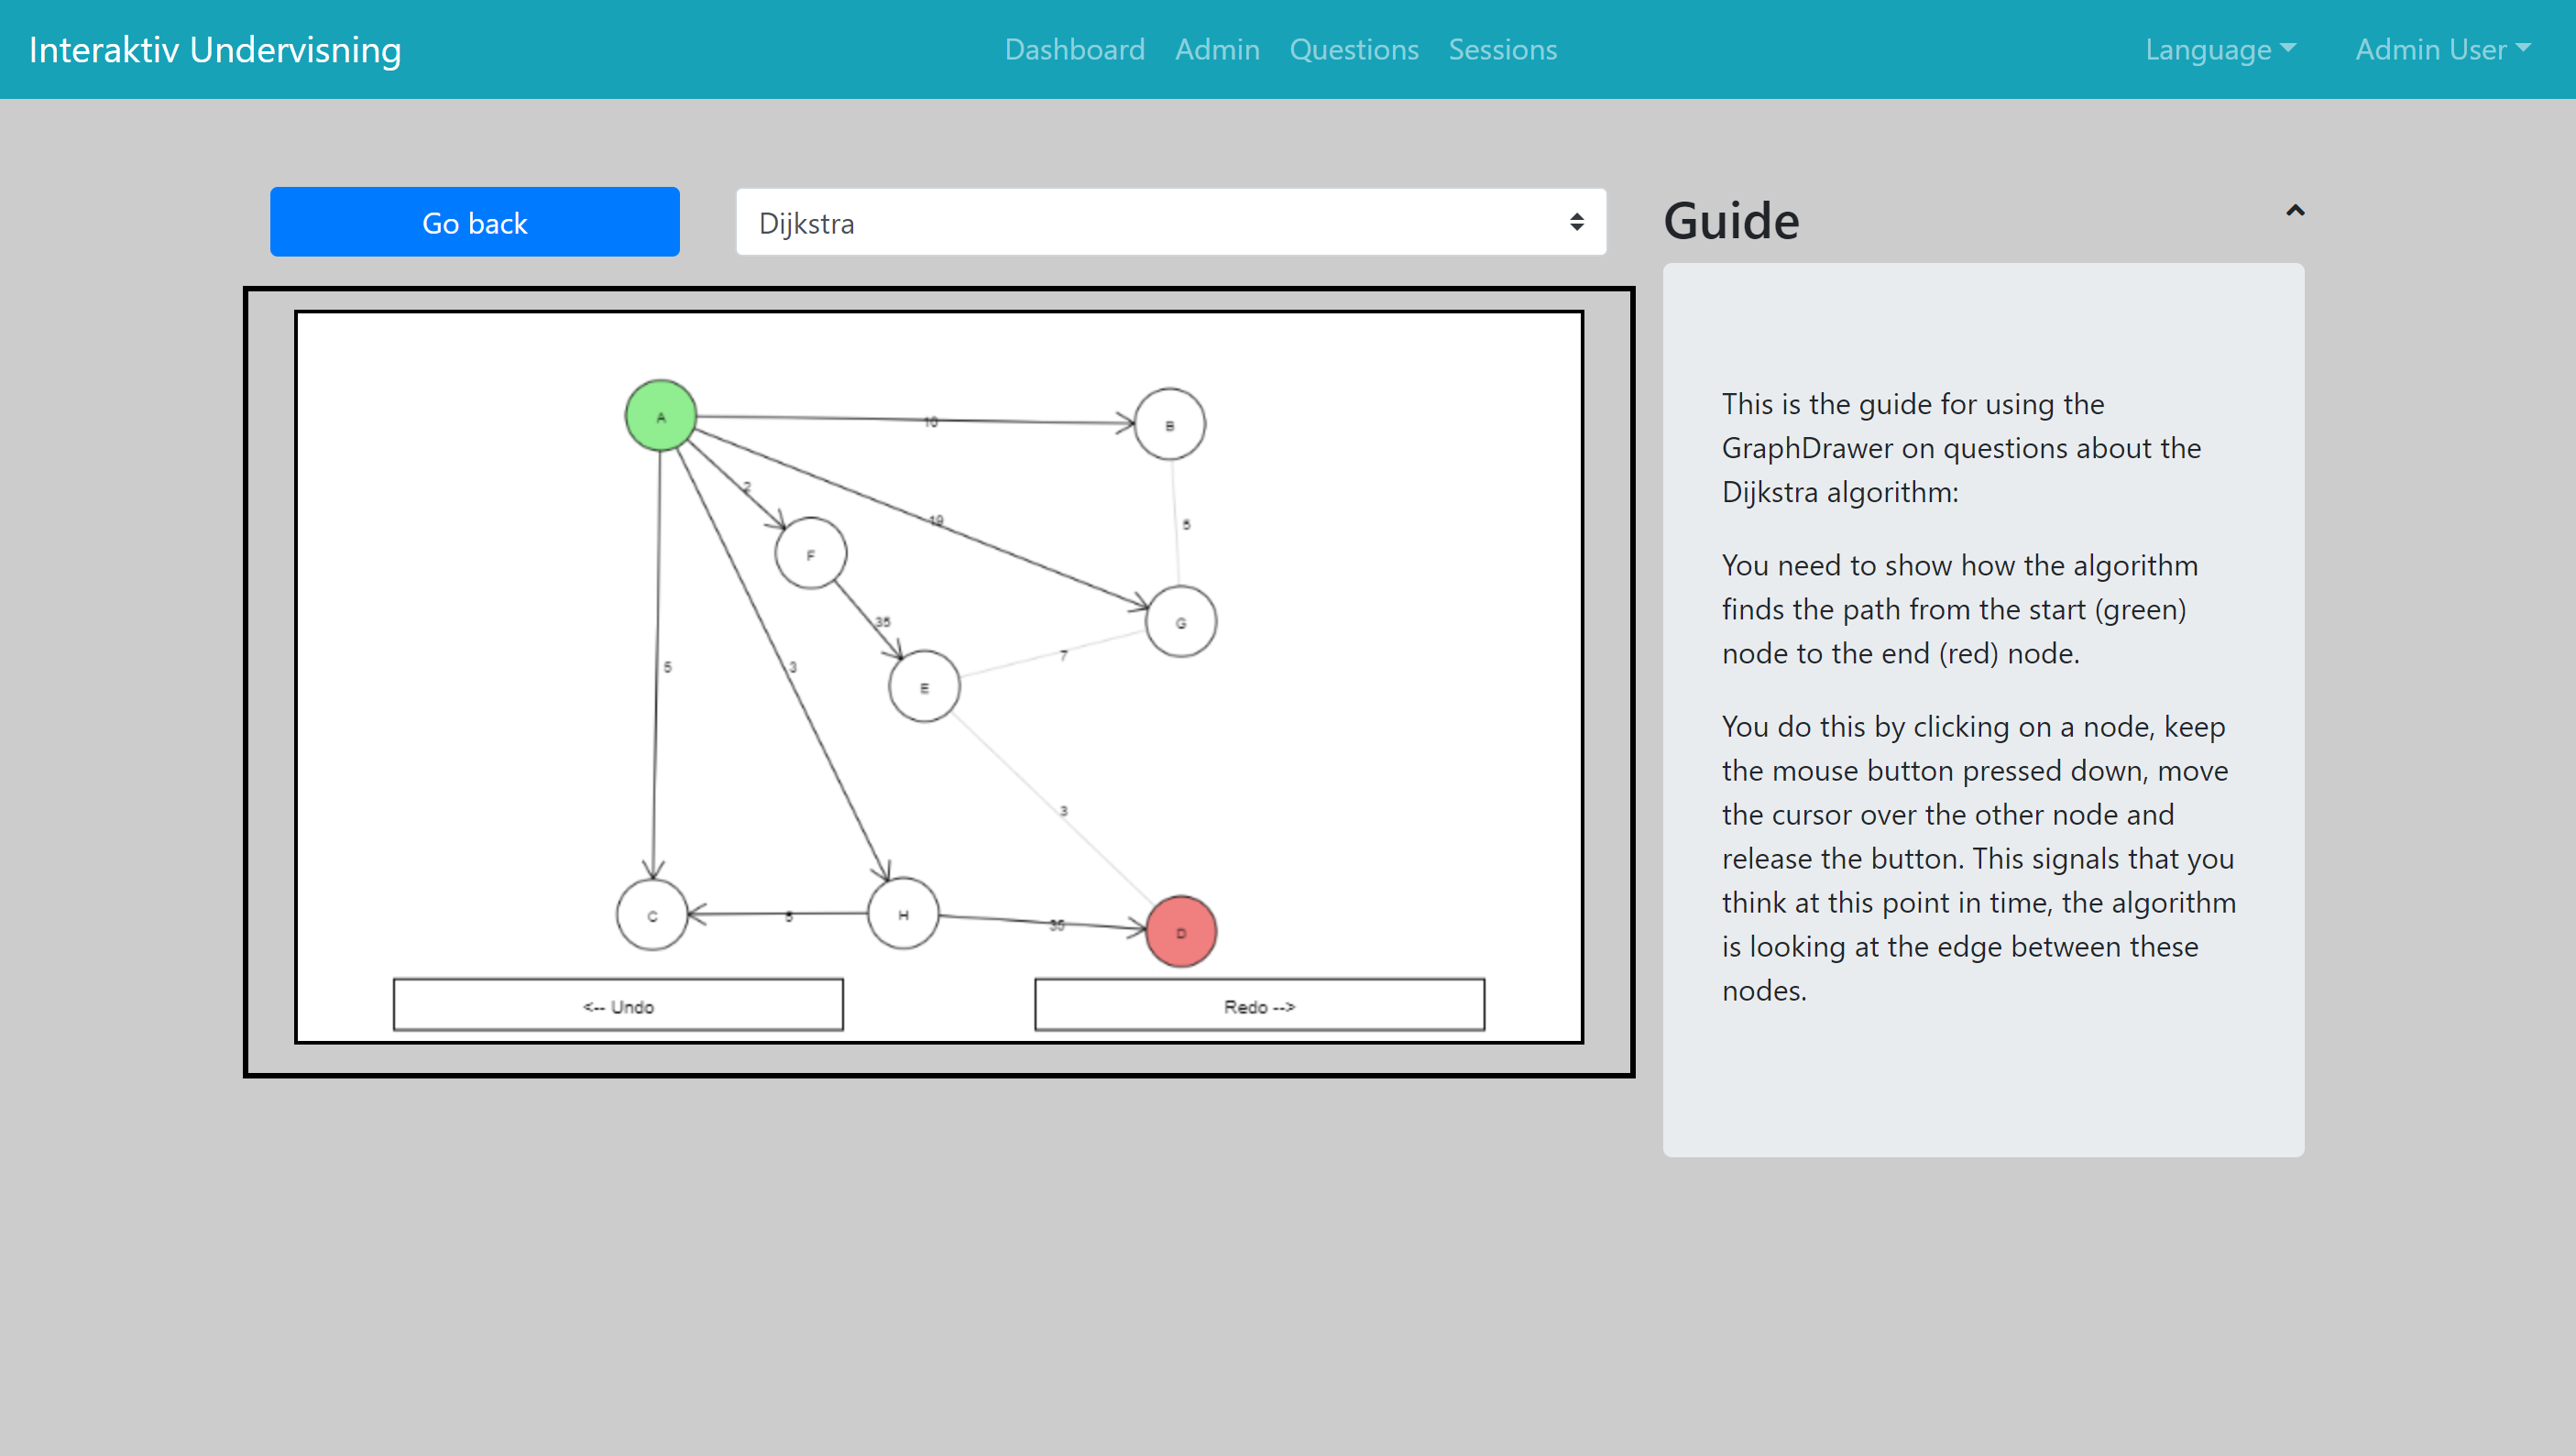
\includegraphics[width=0.80\linewidth]{/userManual/admin/sandbox}
	\caption{This figure displays the sandbox page.}
	\label{fig:sandbox}
\end{figure}